
% to choose your degree
% please un-comment just one of the following
\documentclass[bsc,frontabs,twoside,singlespacing,parskip,deptreport]{infthesis}     % for BSc, BEng etc.
% \documentclass[minf,frontabs,twoside,singlespacing,parskip,deptreport]{infthesis}  % for MInf
\usepackage[utf8]{inputenc}
\usepackage{epigraph}
\usepackage{graphicx} %Added by Songbo
\usepackage{multirow}
\usepackage{rotating} %Added by Songbo
\usepackage{lscape} %Added by Songbo
\usepackage{booktabs}
\usepackage{longtable}
\usepackage{tabu}
\usepackage[options ]{algorithm2e}
\usepackage[ruled,vlined]{algorithm2e}


% Flexible Qoute
\usepackage{epigraph,varwidth}

\usepackage{pifont}% http://ctan.org/pkg/pifont

\usepackage{amssymb}
\usepackage{xcolor}
\newcommand{\bluecheck}{{\color{blue}\checkmark}}
\newcommand{\xmark}{\color{red}\ding{55}}%


\renewcommand{\epigraphsize}{\small}
\setlength{\epigraphwidth}{0.6\textwidth}
\renewcommand{\textflush}{flushright}
\renewcommand{\sourceflush}{flushright}
% A useful addition
\newcommand{\epitextfont}{\itshape}
\newcommand{\episourcefont}{\scshape}


\makeatletter
\newsavebox{\epi@textbox}
\newsavebox{\epi@sourcebox}
\newlength\epi@finalwidth
\renewcommand{\epigraph}[2]{%
  \vspace{\beforeepigraphskip}
  {\epigraphsize\begin{\epigraphflush}
   \epi@finalwidth=\z@
   \sbox\epi@textbox{%
     \varwidth{\epigraphwidth}
     \begin{\textflush}\epitextfont#1\end{\textflush}
     \endvarwidth
   }%
   \epi@finalwidth=\wd\epi@textbox
   \sbox\epi@sourcebox{%
     \varwidth{\epigraphwidth}
     \begin{\sourceflush}\episourcefont#2\end{\sourceflush}%
     \endvarwidth
   }%
   \ifdim\wd\epi@sourcebox>\epi@finalwidth 
     \epi@finalwidth=\wd\epi@sourcebox
   \fi
   \leavevmode\vbox{
     \hb@xt@\epi@finalwidth{\hfil\box\epi@textbox}
     \vskip1.75ex
     \hrule height \epigraphrule
     \vskip.75ex
     \hb@xt@\epi@finalwidth{\hfil\box\epi@sourcebox}
   }%
   \end{\epigraphflush}
   \vspace{\afterepigraphskip}}}
\makeatother

% End Flexiable Qoute


\begin{document}

\title{Building Coherent Open-domain Dialogue Systems Using Neural Networks}

\author{Songbo Hu}

% to choose your course
% please un-comment just one of the following
\course{Artificial Intelligence and Computer Science}
%\course{Artificial Intelligence and Software Engineering}
%\course{Artificial Intelligence and Mathematics}
%\course{Artificial Intelligence and Psychology }   
%\course{Artificial Intelligence with Psychology }   
%\course{Linguistics and Artificial Intelligence}    
%\course{Computer Science}
%\course{Software Engineering}
%\course{Computer Science and Electronics}    
%\course{Electronics and Software Engineering}    
%\course{Computer Science and Management Science}    
%\course{Computer Science and Mathematics}
%\course{Computer Science and Physics}  
%\course{Computer Science and Statistics}    

% to choose your report type
% please un-comment just one of the following
%\project{Undergraduate Dissertation} % CS&E, E&SE, AI&L
%\project{Undergraduate Thesis} % AI%Psy
\project{4th Year Project Report}

\date{\today}

\abstract{
Add abstract later.
}

\maketitle

\section*{Acknowledgements}
Acknowledgements go here. 

\tableofcontents

%\pagenumbering{arabic}

\chapter{Introduction}

\epigraph{When was Alan Turing born? \\
Alan Turing was born on Sunday 13 June 1912. \\
Where was he born? \\
Alan Turing was born in Warrington Lodge. \\
Who is his father? \\
Julius Mathison Turing is Alan Turing's father.\\
When was he born? \\
Julius Mathison Turing was born 9 November 1873. \\
Where? \\
You're at Edinburgh, Scotland.
}{\textit{Songbo and Siri 2020}}

A dialogue system is a conversational agent that can converse with humans in natural language. It can help us solve many tedious tasks effectively or bring entertainment value to our daily life. Recent advances in dialogue systems (such as virtual assistants\cite{alexa,cortana,siri}) enable us to engage in natural conversational interactions with computers. It substantially increases the accessibility of state of the art technologies to people with diverse backgrounds. And for those with impairments, it could transform their daily living into a journey toward capability instead of disability.

Since Alan Turing published his landmark work in 1950\cite{turing1950computing}, the intelligence level of a machine is described as how well the machine is able to fool a human into believing that it, the machine, is a human based on its text responses. If a human is unable to distinguish the difference between the machine from a human, the machine is said to have passed the Turing test. We could say such a machine signifies a significantly high level of intelligence of an AI. It has been the goal for the development of dialogue systems for decades and various attempts have been proposed to pass the Turing test. Recently, advances in neural network based language models enable us to learn entire dialogue models directly from conversational data. Although we improve the performance of neural models by increasing the number of parameters and training with more data, we are still far from our goal. Most of the previous systems have failed to model the longer prior context of the conversation adequately, thereby creating a situation where extended dialogues rapidly become incoherent and unnatural sounding, with repetition being a key problem. 

As I demonstrated in the example conversation at the beginning, humans tend to utilise linguistic patterns, such as anaphora and sluicing to reduce repetitions. In contract, dialogue systems rarely produces pronouns and unable to model elided construction therefore produce unnatural speech in the context. For example, in order to answer the second question ("Where was he born?"), humans are able to interpret the anaphora (He refers to Alan Turing.) and produce a short answer (In Warrington Lodge.). Compared to human's responses, Siri's responses are heavy and verbose. The challenge for Siri, and many other dialogue systems, is to know when such an answer conveys the intended content, and when it doesn't. The system has to make a decent decision on when content can be elided while still ensuring that the user can easily interpret the system's message and retrieve that message accurately. In addition, a wrong interpretation of a question could lead to an unhelpful and diverged response. Siri fails to understand the context to parse fragments and interpret the sluicing in the final question. The misunderstanding of the context leads to a completely unhelpful and incoherent response. The main reasons of this unnaturalness for Siri is the lack of reliable systematic analysis of such linguistic patterns and the inadequate representation of the context. It is a problem which need to be adequately addressed before our agents could look forward to attempting the Turing test. This is the main motivation for this project.

In this section, we will briefly review the recent development of dialogue systems. Specifically, we will discuss two types of dialogue systems: the chit-chat dialogue systems (known as chat bots), and the task-oriented dialogue systems.  We will focus on machine learning approaches to developing such systems, rather than the use of hand-crafted rules, since the former methods are now dominant and the latter are highly brittle and restricted to toy domains. We will discuss their architectures, pros and cons, and their main limitations to achieve coherent open-domain conversations. The majority of this thesis is about how to create an environment for neural models to learn linguistic patterns within coherent extended dialogues and how to integrate these models into the existing dialogue systems. It constitutes a first step towards modelling coherent open-domain conversations and will potentially enable the existing dialogue systems utilising valuable linguistic information to produce coherent responses.

\section {A Brief Review of Existing Dialogue Systems}

\subsection{The Chit-chat Dialogue System}

The chit-chat dialogue systems are usually called chatbots. These systems are designed and implemented to carry extended conversations with the goal of mimicking the ‘chats’ characteristic of informal human-human interaction\cite{jurafsky2019speech}. They are mainly aiming to provide entertainment value. Existing chatbots majorly fall into the following subcategories: the rule-based systems, the corpus-based systems, as will be discussed in order below.

\subsubsection*{The Rule-based Systems}

Instead of letting machines to learn the conversation strategy from human behaviours, we could ask humans to encode these human intelligence directly as rules and ask machines to interpret them. Dialogue agents could use these rules to generate dialogue utterances effectively. Normally, a message input will be processed by a set of carefully pre-defined rules e.g., a key-word look-up dictionary, if-else conditions, or more sophisticated machine learning classifiers\cite{jiweilithesis}. Consequently, the dialogue agent would produce a natural language response by outputting an utterance in storage, manipulating the input message or selecting some related historical contexts based on these rules.

\begin{figure}[h]
    \centering
    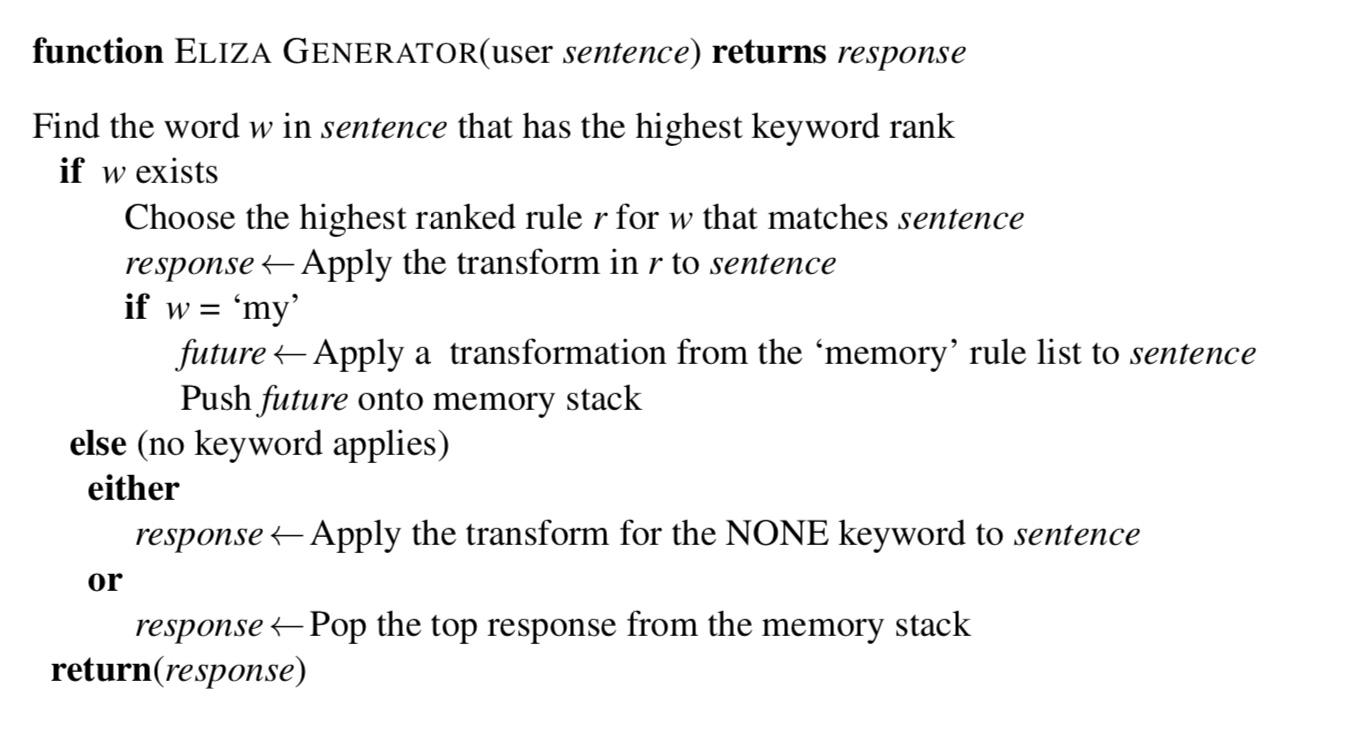
\includegraphics[width=0.9\textwidth]{elizarule.jpeg}
    \caption{A simplified sketch of the ELIZA algorithm.}
    \label{fig:elizarule}
\end{figure}

There are many well-known rule-based dialogue systems in history, such as ELIZA\cite{weizenbaum1966eliza}, ALICE\cite{wallace1995artificial}. There are also languages such as Artificial Intelligence Markup Language(AIML), which provides an effect tool to write sophisticated conversations logic in a machine-readable format\cite{wallace1995artificial}.

The development of rule-based systems is an important milestone in developing modern dialogue systems. They demonstrate how easy to fool a user into thinking there is intelligence in the machines behaviour when in fact there is no understanding and comprehension at all. Consequently, their drawbacks are obvious: rule-based systems predominantly rely on the set of pre-defined rules and these rules have to be carefully designed and implemented. Building a sophisticated rule-based system is very expensive because the number of these rules escalates rapidly. Rule-based systems do not have the ability to understand human languages and generate meaningful natural language utterances\cite{jiweilithesis}. Consequently, they are very brittle and only able to conduct very superficial conversations. Despite the lack of intelligence, even with the recent rapid development of large fancy neural network architecture and increasing number of conversational corpora, these rule-based dialogue systems could always provide a very strong baseline.

\subsubsection*{The Corpus-based Systems}

Coding conversation logics manually is astronomically expensive and infeasible for many applications. Corpus-based dialogue system could potentially alleviate this issue by mining human-human conversations, or sometimes mining the human responses from human-machine conversations, instead of using hand-built rules. These data-driven approaches are becoming widely popular due to the increasing computing power and the creation of large scale conversational dataset. 

There are two common architectures for such system: information retrieval (IR), and machine learned sequence transduction. Due to the limitation that IR-based chatbots can only mirror training data, it is often to treat response generation as a machine translation task which transduces from the user’s prior turn to the system’s turn. This method offers the promise of scalability and language-independence, together with the capacity to capture contextual dependencies in a way not possible with IR-based approaches.

\begin{figure}[h]
    \centering
    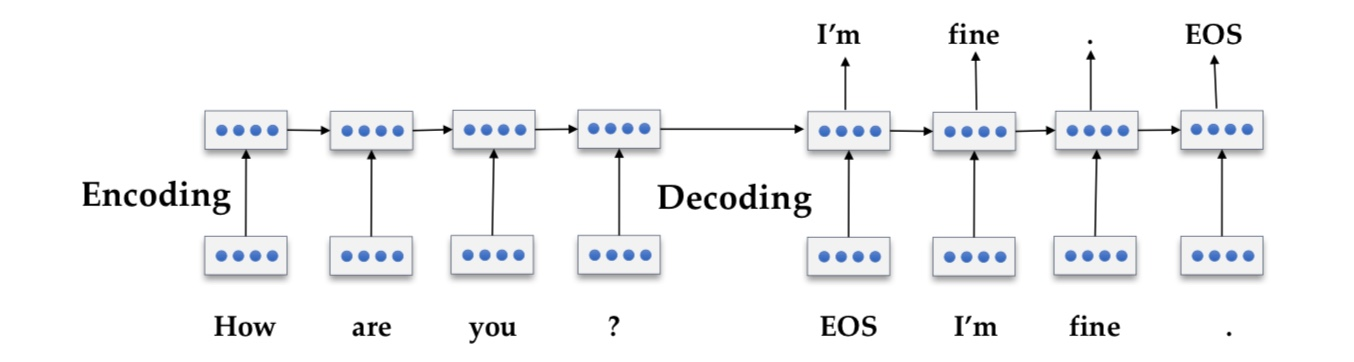
\includegraphics[width=0.9\textwidth]{seq2seq.jpeg}
    \caption{A sequence to sequence model for neural response generation.\cite{jurafsky2019speech}}
    \label{fig:seq2seq}
\end{figure}

This idea was firstly developed by Ritter et al\cite{ritter2011data}. (cited in Jurafsky and Martin\cite{jurafsky2019speech}) using phrase-based machine translation to translate a user turn to a system response. In 2015, transduction models for response generation were modelled using encoder-decoder (seq2seq) models\cite{shang2015neural,strub2017end,sordoni2015neural}. However, the simple seq2seq generation architecture is unable to model the prior context of the conversation. Serban et al\cite{serban2016building} suggests a hierarchical (HRED) model that summarizes information over multiple prior turns. This model consists of two recurrent neural networks (RNNs) stacked on top of each other: one is a sentence-level RNN which encodes each utterance into a fixed length vector, while a conversation-level RNN takes each utterance vector as input and outputs a vector that summarizes the conversation so far. The vector is mapped back to text using a recurrent decoder. This gives a way for the previous information to be passed to future turns as hidden states\cite{lowe2017training}.

\begin{figure}[h]
    \centering
    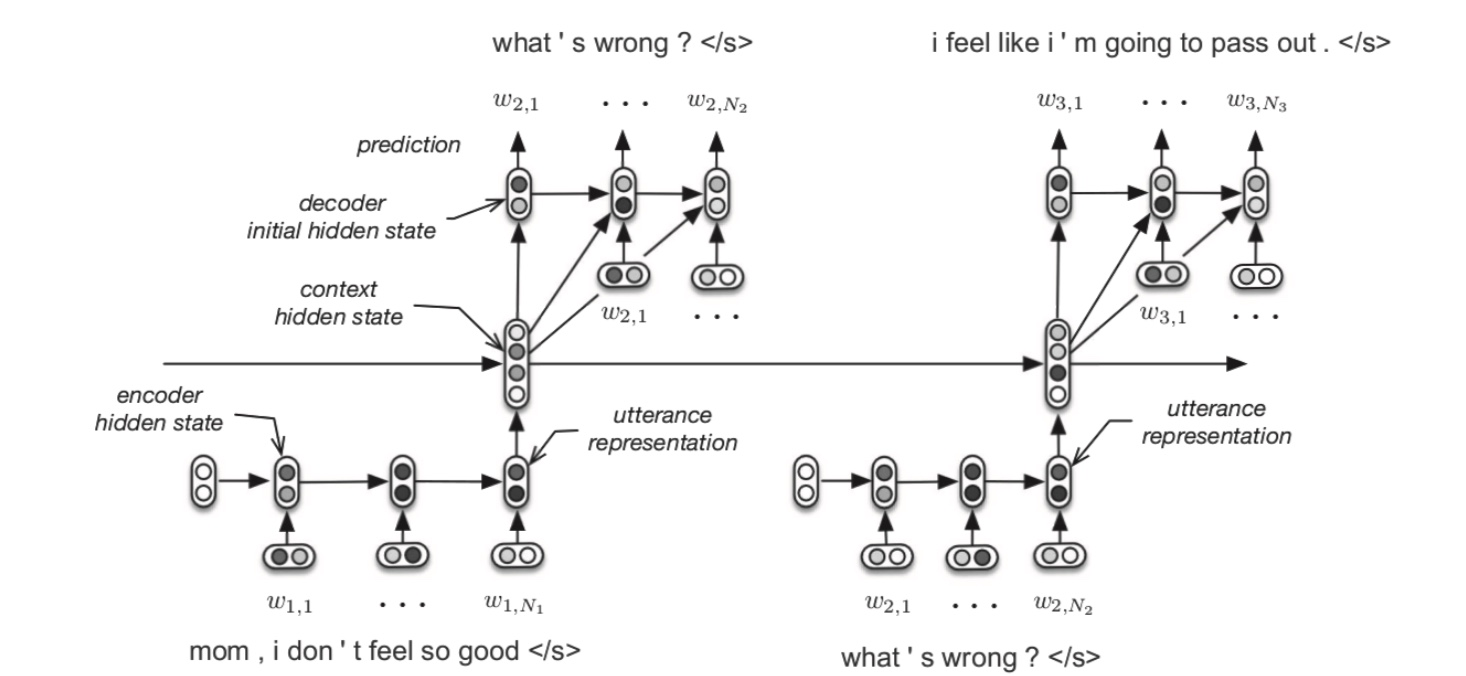
\includegraphics[width=0.9\textwidth]{HERD.jpeg}
    \caption{The computational graph of the HRED architecture for a dialogue composed of three turns.}
    \label{fig:HERD}
\end{figure}

However, even if one has access to an enormous dataset for training, there is still a significant proportion of unseen dialogue states. Techniques, such as smoothing, can only help to a limited extent, because of the radical extent to which data is sparse. Consequently, generating responses using end-to-end methods tends to generate generic, uninformative and non-coherent replies (e.g., generating ``I don’t know." regardless of the context). In addition, encoder-decoder response generators focus on generating single responses, instead of forming a coherent continuous conversation\cite{jurafsky2019speech}. Humans could easily notice these unnatural and mechanical responses (e.g. the Siri conversation above). Techniques, such as Reinforcement learning (RL)\cite{li2016deep} and adversarial networks\cite{li2017adversarial}, can be used to address this issue.

\subsection{The Goal-oriented Dialogue System}

 Goal-oriented dialogue systems are sometimes also called task-based dialogue systems, in which they converse with users to help complete tasks like making a restaurant reservation, booking a hotel or setting up an alarm. Famous examples of such agents are digital assistants (Siri, Alexa, Google Home, Cortana, et.)\cite{siri,alexa,googlehome,cortana} which can be viewed as a combination of chatbots and goal-oriented dialogue systems. With the power of cloud computing and internet of things technologies, these conversations AIs are changing our daily life and developing a 10 billion pounds worth industry\cite{chatbotmarket}. Here, I would like to introduce the architectures of existing statistical spoken dialogue systems (hereafter SDSs) and their main challenges to perform coherent conversations in an open domain. 

\begin{figure}[h]
    \centering
    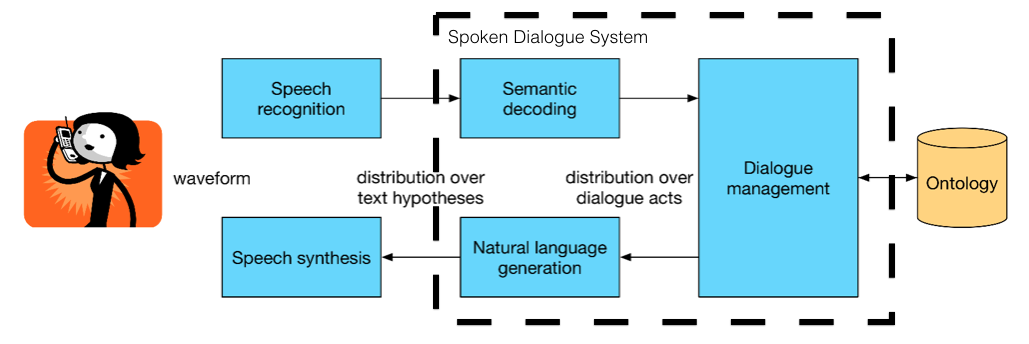
\includegraphics[width=0.80\textwidth]{sds.png}
    \caption{Architecture of a Spoken Dialogue System.\cite{gasic}}
    \label{fig:sds}
\end{figure}

Current SDSs have three key components which are shown as Figure\ref{fig:sds}. A semantics decoder decodes the meaning in utterances into dialogue acts which describe the current intention of the user, for example, confirm(food=Korean). Then, a dialogue manager, which usually consists of a belief tracker and a policy network, will keep track of the belief states and produce a dialogue act as the response. The dialogue manager treats dialogue generation as a partially observable Markov decision process (POMDP)\cite{williams2007partially,young2013pomdp,young2010hidden} which explicitly models the uncertainty natural of human conversations with Bayesian methods. Such framework provides robustness against the errors created by the speech recognition. Later a semantic encoder (natural language generator) will map this act back into a natural language response.

However, keeping track of the belief states under such a framework presents a tough challenge. Exact model representation is infeasible due to the limitation of computational complexity\cite{young2013pomdp}. Carefully constructed approximation and additional independent assumption are needed. For example, if we are willing to find an expensive 5-star hotel in the city center, in order to make the inference practical, we have to assume that there is no relation between a hotel is expensive and it is a 5-star hotel. It is clearly not true. In addition, as shown in Figure\ref{fig:sds}, pre-defined ontology is needed in order to keep track of the dialogue state. This makes the existing dialogue system infeasible to perform conversations in an open-domain. One research direction would be building a SDS which can support a natural conversation about any topic within a wide coverage Knowledge Graph (KG). This forms the definition of an open-domain spoken dialogue system\cite{opendomain}.




\section {Thesis Outline}

In this thesis, we mainly focus on creating a framework in which neural models could learn linguistic patterns within in extended coherent dialogues.

Firstly, we explore how to build such a framework by designing, collecting and annotating a conversational dataset. This dataset consists of extended coherent dialogues of questions and responses. These dialogues should describe the relations within a knowledge graph with clear links between the phrases in the questions to nodes in a knowledge graph. Secondly, we analyse the collected dataset statistically in order to investigate how human behave differently under different context in different domain. Later, we will introduce a proposed neural model to model these linguistic patterns and how the existing dialogue systems could benefit from such a model.

We start off by providing background knowledge on available corpora to train dialogue models and how to evaluate these dialogue models in Chapter 2. In chapter 3 and chapter 4, we will describe the design and creation of our framework in details and perform analysis to figure out the common patterns within these dialogues. Chapter 5 will introduce our proposed neural models and methods in order to model coherent dialogues with neural networks. We will briefly summarize our findings and mention some further work in Chapter 6.

\chapter{Background}

In this chapter, we investigate the existing resources and frameworks to build a neural dialogue model and summarize the popular evaluation metrics for the dialogue modeling task.

\section{Corpora for Training Dialogue Models}

Humans perform dialogues with different purposes, under different situations and in different medias. There is a vast amount of data available documenting human communications. Some of these data is collected as corpora and these corpora can be classified into different categories. Each category has different characteristics, utilities and applications. In order to make the most of the available resources, we discuss the important distinctions between each type of dialogue corpora: whether the corpus features constrained or unconstrained dialogues; whether a corpus is written, spoken; whether a corpus features human-human interactions or human-machine interactions. Afterwards, I give a brief summary about current public available corpora.

\subsection{Chit-chat or Goal-oriented Corpora}

People use different languages for different purposes. We may want to call an airliner to book a ticket or chat with our friends to share our brilliant ideas. The purpose and motivation of our conversation will have a significant influence on the language we use. Similarly, the way in which a dialogue corpus is collected can also have a significant influence on the model we built from. Some conversations are relatively causal, informal and unconstrained, which we usually call them chit-chats. There are many chit-chat corpora and most of them are aiming to mimic spontaneous and unplanned spoken interactions between humans. Consequently, they are also referred as Spontaneous (Unconstrained) Corpora\cite{serban2018survey}. Another large proportion of the existing corpora focus on a particular topic or intend to solve a specific task. In such situations, the task or topic is pre-specified and participants are discouraged from deviating from the topic. We refer to these as Task-Oriented or Constrained Dialogue Corpora.

Spontaneous corpora usually contains richer grammar and vocabularies, which reflect our daily commutation well. However, such corpora are usually in plain text with less informative annotations. Consequently, people usually train models with end-to-end methods suing those corpora. Such setting could reduce the interpretability of models' reasoning and pose additional challenges to models' evaluation, which we will discuss in later section. 

For constrained dialogues, some experimental conditions in which dialogues were collected can result in unnatural behaviours. Consequently, dialogues in goal-oriented corpora usually don't bear a close resemblance to our daily commutations and do not correlate well to the true typical dialogue patterns in natural conversations. Therefore, all experimental conditions have to be carefully designed to make sure that the conversations have the desired properties we are looking for. Not only the experiment instruction, but also many other factors (e.g. the demographics of the participants\cite{ai2007comparing,young2013pomdp}) could significantly influence the data we collected. It is generally hard to do before we actually run the experiment. Designing a constrained dialogues is particularly challenging, 

\subsection{Written, Spoken or Multi-modal Corpora}

Another important distinction between dialogue corpora is whether participants interact through written language, spoken language, or in a multi-modal setting (e.g. using both speech and visual modalities). Written and spoken language differ from each other and have substantially different linguistic properties. Spoken language tends to be informal, containing less information per utterance and have more pronouns than written language\cite{carter2006cambridge,biber2001diachronic}.

Similarly, dialogues involving visual and other modalities differ from dialogues without these modalities\cite{serban2015survey,duncan1983charles}. When a visual modality (e.g. body language, eye contact, hand motions) is available, such non-verbal information could influence the distributions of many linguistic properties significantly\cite{gibson1963perception,lord1974perception,cooper1974control,chartrand1999chameleon,de2013speaker}. Consequently, we should take all those factors in to account in designing our own corpus.

\subsection{Human-Human or Human-Machine Corpora}

Another salient distinction between dialogue corpora resides in the types of interlocutors. Conversations between two humans are totally different from conversations involving machines.

This distinction is important because current computer dialogue systems exhibits very different traits than human-human dialogue\cite{doran2003comparing}. Machines are significantly constrained and normally produce less changeable dialogues. These systems do not produce the same distribution of possible responses as humans do under the same conditions. In addition, human-machines dialogues contains different type of errors and the turn-taking in these dialogues are much more predictable\cite{williams2007partially}. Consequently, in order to learn natural conversations, it is not sensible to learn from human-machine corpora, as the trained dialogue system would simply learn to approximate the policy of the the dialogue system\cite{serban2018survey}.

Another possible experiment setting is called Wizard-of-Oz experiments\cite{bohus2008sorry,petrik2004wizard,budzianowski2018multiwoz,eric2019multiwoz}. In Wizard-of-Oz experiments, a human thinks he/she is speaking to a machine dialogue system, but a human is in fact controlling the dialogue system. This is very similar to Turing's test, but in reversed order. Conversations in such setting are likely to have similar distributions as the the situation when the dialogue system has nearly human-level performance. This can encourage machines to learn from human intelligence and achieve comparable performance when the behaviour of another human participant is not seriously different.  

\subsection{Available Dialogue Corpora}

Covering all available corpora for training dialogue models is infeasible, therefore, we would only focus on three popular categories: Human-Human spontaneous dataset, human-human constrained dataset and human-machine dataset. I would like to give examples which are well-known or directly related to this project. Table\ref{tab:HHSTable} and Table\ref{tab:HHGoal} summarize those available corpora and compare the key features between them.

\subsubsection{Human-human Spontaneous Corpora}

People talk to each other for entertainment. Here, we classify all corpora that participants talk without a pre-defined objective as spontaneous(chit-chat) corpora. Normally, the domain of these corpora would be unconstrained.

Firstly, I would like to introduce some important spoken spontaneous corpora. The Switchboard dataset\cite{godfrey1992switchboard} is one of the most influential spoken corpora. This dataset consists of approximately 2,500 dialogues from phone calls, along with word- by-word transcriptions, with about 500 different speakers. A computer-driven robot operator system introduced a topic for discussion between two participants, and recorded the resulting conversation. About 70 casual topics were provided, of which about 50 were frequently used. The corpus was originally designed for training and testing various speech processing algorithms; however, it has also been used for a wide variety tasks. Another important dataset is the British National Corpus (BNC)\cite{leech1992100}), which contains approximately 10 million words of dialogue. These were collected in a variety of contexts ranging from formal business or government meetings, to radio shows and phone-ins. Although most of the conversations are spoken in nature, some of them are also written. BNC covers a large number of sources, and was designed to represent a wide cross-section of British English from the late twentieth century. The corpus also includes part-of-speech (POS) tagging for every word. The vast array of settings and topics covered by this corpus renders it very useful as a general-purpose spoken dialogue dataset.

Instead of using spoken language, there are also numerous corpora based on different medias. With the enormous increase of Internet users all over the world and the rapid development of social media industry, a tremendous amount of conversations are recorded on the Internet. For example, online chatroom seems to be a good source o f conversations. NPS Internet Chatroom Conversations Corpus\cite{forsythand2007lexical}, which consists of 10,567 English utterances gathered from age-specific chat rooms of various online chat services from October and November of 2006. This copus is one of the first corpora uses Internet to be its media of communication. Several corpora of micro-blogging conversations have also been collected, such as the Twitter Corpus\cite{ritter2010unsupervised}, which contains 1.3 million post-reply pairs extracted from Twitter. The corpus was originally constructed to aid in the production of unsupervised approaches to modeling dialogue acts. Larger Twitter corpora have been collected. The Twitter Triples Corpus\cite{sordoni2015neural} is one such example, with a described original dataset of 127 million context-message-response triples. Not only for English, but also for many other languages, a large micro-blogging dataset has been created, such as, the Sina Weibo Corpus\cite{shang2015neural}, which contains 4.5 million post-reply pairs in Chinese.

These corpora collected from the Internet has an enormous amount of typos, slang, and abbreviations. Particularly for twitter, due to the 140-character limit in this dataset, tweets are often very short and compressed\cite{serban2018survey}. Another challenge is that Twitter conversations often rely on implicit context (e.g. they refer to recent public events outside the conversation). In order to learn effective responses for such conversations, a dialogue agent must infer the news event under discussion by referencing some form of external knowledge base. This would appear to be a particularly difficult task.

% Please add the following required packages to your document preamble:
% \usepackage{multirow}
% \usepackage{lscape}
\begin{landscape}
\begin{table}[]
\begin{tabular}{|l|l|r|l|l|l|l|}
\hline
Type                                                                                          & Name                                                                                                                            & Year                      & Source        & \begin{tabular}[c]{@{}l@{}}Number \\ of Dialogues\end{tabular} & \begin{tabular}[c]{@{}l@{}}Number\\ of Words\end{tabular} & Annotation                                                                                                 \\ \hline
\multirow{9}{*}{\begin{tabular}[c]{@{}l@{}}Human-Human \\ spontaneous\\ Corpora\end{tabular}} & Switchboard\cite{godfrey1992switchboard}                                                                                        & 1992                      & Spoken        & 2,400                                                          & 3M                                                        &                                                                                                            \\ \cline{2-7} 
                                                                                              & British National Corpus\cite{leech1992100}                                                                                      & 1992                      & Spoken/Writen & 854                                                            & 10M                                                       & Part of speech tags                                                                                        \\ \cline{2-7} 
                                                                                              & NPS Chat Corpus\cite{forsythand2007lexical}                                                                                     & 2007                      & Online Chat   & 704                                                            & 100M                                                      & \begin{tabular}[c]{@{}l@{}}Dialogue acts and\\ Part of speech tags\end{tabular}                            \\ \cline{2-7} 
                                                                                              & Twitter Corpus \cite{ritter2010unsupervised}                                                                                    & 2010                      & Microblog     & 1.3M                                                           & 125M                                                      &                                                                                                            \\ \cline{2-7} 
                                                                                              & Twitter Triple Corpus\cite{sordoni2015neural}                                                                                   & 2015                      & Microblog     & 4232                                                           & 65K                                                       &                                                                                                            \\ \cline{2-7} 
                                                                                              & DailyDialog\cite{li2017dailydialog}                                                                                             & \multicolumn{1}{l|}{2017} & Online Chat   & 13K                                                            & 15M                                                       & Emotion                                                                                                    \\ \cline{2-7} 
                                                                                              & \begin{tabular}[c]{@{}l@{}}The Cambridge and Nottingham \\ Corpus of Discourse in English\cite{mccarthy1998spoken}\end{tabular} & \multicolumn{1}{l|}{1998} & Spoken        & -                                                              & 5M                                                        & \begin{tabular}[c]{@{}l@{}}Relationship between\\ speakers and interaction type\end{tabular}               \\ \cline{2-7} 
                                                                                              & \begin{tabular}[c]{@{}l@{}}D64 Multimodal Conversation\\  Corpus\cite{oertel2013d64}\end{tabular}                               & \multicolumn{1}{l|}{2013} & Video         & 2                                                              & 70K                                                       & \begin{tabular}[c]{@{}l@{}}Physical head, torso and\\  arm motion\end{tabular}                             \\ \cline{2-7} 
                                                                                              & Topical Chat\cite{Gopalakrishnan2019}                                                                                           & \multicolumn{1}{l|}{2019} & Online Chat   & 10784                                                          & 4M                                                        & \begin{tabular}[c]{@{}l@{}}Links between plain text \\ grounded knowledge\\  and conversation\end{tabular} \\ \hline
\end{tabular}
\caption{Example uman-Human spontaneous dataset}
\label{tab:HHSTable}
\end{table}
\end{landscape}

\subsubsection{Human-Human Goal-oriented dataset}

For many corpora, the topic of the conversation specified beforehand and participants are discouraged from deviating off-topic. Most of the participants in the conversations are aiming to solve a specific task or help the other participants to solve the task. Consequently, these corpora are slightly less general and natural because we, as the task designer, introduce additional biases. These biases will influence the distributions of the linguistics properties which should be carefully considered. Such setting also brings huge benefits. It makes extrinsic possible and dialogue states inferenecs easier since all participants share the same prior knowledge. Here, I would like to discuss some common types of tasks for the existing corpora.

Several corpora focus on task planning or path-finding through the collaboration of two interlocutors. In these corpora typically one person acts as the decision maker and the other acts as the observer. A well-known example of such a dataset is the HCRC Map Task Corpus\cite{anderson1991hcrc}, that consists of unscripted, task-oriented dialogues that have been digitally recorded and transcribed. In the corpora, each participants must collaborate verbally to reproduce a route from one of the participant’s map to the map of another participant. 

Another theme recurring among these corpora is the appearance of persuasion or debate tasks. These can involve general debates on a topic or tasking a specific interlocutor to try to convince another interlocutor of some opinion or topic. Generally these datasets record the outcome of how convinced the audience is of the argument at the end of the dialogue or debate. The Intelligence Squared Debate Dataset\cite{zhang2016conversational} covers the “Intelligence Squared” Oxford-style debates taking place between 2006 and 2015. The topics of the debates vary across the dataset, but are constrained within the context of each debate. Speakers are labeled and the full transcript of the debate is provided. Furthermore, the outcome of the debate is provided (how many of the audience members were for the given proposal or against, before and after the debate).

Another popular task is to perform  Question-Answering tasks grounding on external knowledge. Many researchers are aiming to creates a mini-game where two players ask and answer sequential questions in turns and form a dialogue aiming to accomplish some pre-specified tasks. Instead of direct question-and-answering with common knowledge, they provide external grounding knowledge for each participants. By doing so, we could reduce the influences of participants' own prior knowledge in the dialogue state representations.

GuessWhat\cite{de2017guesswhat} is a two-player game where the goal is to identify an object in a complex visual scene by asking a sequence of yes/no questions. There are 150k human-human dialogues collected which contains 821k questions together with YES/NO answers. This is one of the common tasks for these minigames, which is usually tcalled visual question answering (VQA) task. There are many efforts towards this direction\cite{strub2017end,shekhar2017foil,reddy2019coqa,zhou2018dataset,de2017guesswhat,das2017visual,das2017learning}, in which they try to model visually grounded conversations using different machine learning paradigms (including RL) in a question answering setting. However, the imperfect performance of the image encoding network leads to a poor RL policy, which is the bottleneck of the whole system. Instead of learning the best conversational strategy, the model learns to find the most effective protocol by utilizing the strength of the answering network. This protocol will clearly not produce natural conversations.

Instead of grounding conversations on images, Reddy et al.\cite{reddy2019coqa} proposed a conversational question answering challenge (CoQA) which contains question answering conversations in natural language grounded on a short paragraph with its supporting evidence. However, the top models on the leader board surpass human performance. Even if we ignore the sequence labelling nature of the task, which humans may under-perform, it is clear that even the state of the art neural model would not achieve human intelligence on these kinds of natural language understanding tasks. The results above demonstrate that whatever representations these models learn, they are fundamentally different from what we are expecting. This emphasises the importance of the interpretability of a network's reasoning. We need a framework in which we can perform controlled evaluation, because only then we can justify its decisions.

To the best of our knowledge, there is no publicly available corpus on training coherent open-domain dialogue models. As I argued above, we need ground knowledge which both humans and machines could interpret effectively. In chapter 3, I will demonstrate that knowledge graph could be a choice as the external knowledge. 
% Please add the following required packages to your document preamble:
% \usepackage{multirow}
% \usepackage{graphicx}
% \usepackage{lscape}
\begin{landscape}
\begin{table}[]
\resizebox{660}{!}{%
\begin{tabular}{|l|l|r|l|l|l|l|}
\hline
Type                                                                                           & Name                                                              & Year                      & Source              & \begin{tabular}[c]{@{}l@{}}Number \\ of Dialogues\end{tabular} & \begin{tabular}[c]{@{}l@{}}Number\\ of Words\end{tabular} & Description                                                                                                                                                                              \\ \hline
\multirow{6}{*}{\begin{tabular}[c]{@{}l@{}}Human-Human\\ Goal-oriented\\ Corpora\end{tabular}} & HCRC Map Task Corpus\cite{anderson1991hcrc}                       & 1991                      & Spoken              & 128                                                            & 147K                                                      & \begin{tabular}[c]{@{}l@{}}Dialogues from HLAP Task in which \\ speakers must collaborate verbally\\ to reproduce on one participants \\ map a route printed on the others.\end{tabular} \\ \cline{2-7} 
                                                                                               & Intelligence Squared Debate Dataset\cite{zhang2016conversational} & 2016                      & Debates             & 854                                                            & 10M                                                       & \begin{tabular}[c]{@{}l@{}}Various topics in Oxford-style debates,\\  each constrained to one subject. \\ Audience opinions provided pre- and\\  post-debates.\end{tabular}              \\ \cline{2-7} 
                                                                                               & GuessWhat                                                         & 2017                      & Mini Game           & 160K                                                           & 4M                                                        & \begin{tabular}[c]{@{}l@{}}Identify an object in a complex visual\\ scene by asking a sequence of \\ yes/no questions\end{tabular}                                                       \\ \cline{2-7} 
                                                                                               & Complex Sequential Question Answering\cite{2018complex}           & 2010                      & Semi-auto Generated & 169K                                                           &                                                           & \begin{tabular}[c]{@{}l@{}}Sequential Question Answering Utterance\\ generated based on human defined templet\end{tabular}                                                               \\ \cline{2-7} 
                                                                                               & CoQA\cite{reddy2019coqa}                                          & 2019                      & QA Chat             & 8K                                                             &                                                           & \begin{tabular}[c]{@{}l@{}}Question Answering Conversation grounded \\ on short paragraph. Labeled with text spans\\ as supporting evidence.\end{tabular}                                \\ \cline{2-7} 
                                                                                               & QuAC\cite{choi2018quac}                                           & \multicolumn{1}{l|}{2018} & QA Chat             & 14K                                                            & 5.6M                                                      & \begin{tabular}[c]{@{}l@{}}Question Answering Conversation grounded\\ on wikipeida text. Labeled with text spans\\ as supporting evidence. Annotated with\\  dialogue acts.\end{tabular} \\ \hline
\end{tabular}%
}
\caption{Example Human-Human Goal-oriented Corpora}
\label{tab:HHGoal}
\end{table}
\end{landscape}

\subsubsection{Human-Machine Corpora}

Most of the Human-Machine Corpora are Goal-oriented. Humans usually talk to machines in order to accomplish tasks or enquiry information. The ATIS (Air Travel Information System) Pilot Corpus\cite{hemphill1990atis} is one of the first human-machine corpora. It consists of interactions, lasting about 40 minutes each, between human participants and a travel-type booking system, secretly operated by humans. This dataset contains 1041 utterances. The Carnegie Mellon Communicator Corpus\cite{bennett2002carnegie} also contains human-machine interactions with a travel booking system. It is a medium-sized dataset of interactions with a system providing up-to-the-minute flight information, hotel information, and car rentals. Conversations 
with the system were transcribed, along with user’s comments after the interaction.

Instead of making queries or making reservations, people also talk to machines for other purpose. The DIALOG mathematical proof dataset\cite{wolska2004annotated} is a Wizard-of-Oz dataset involving an automated tutoring system that attempts to advise students on proving mathematical theorems. This is done using a hinting algorithm that provides clues when students come up with an incorrect answer. At only 66 dialogues, the dataset is very small, and consists of a conglomeration of text-based interactions with the system, as well as think-aloud audio and video footage recorded by the users as they interacted with the system. The latter was transcribed and annotated with simple speech acts such as “signaling emotions” or “self-addressing”.


\section{Dialogue Model Evaluation}

Evaluating dialogue models is one of the most challenging aspects of building dialogue systems. Dialogue systems are generally evaluated by humans, however, human evaluation is very time consuming and expensive. Although user satisfaction is our ultimate goal for building dialogue systems, it is often necessary to optimize the performance on some automatic metrics for multiple times prior to release. It is inefficient to run experiments with real user during the development circle. In this section, I will briefly investigate commonly used approaches for dialogue system evaluation in three categories: Intrinsic Evaluation, Extrinsic Evaluation and Human Evaluation, and discuss the pros and cons of each approach.

\subsection{Intrinsic Evaluation}

\subsubsection{Word Overlap Metrics}

As I mentioned in Chapter 1, modelling dialogues could be views as a machine translation task. Consequently, we may borrow  machine translation evaluation metrics, such as BLEU scores\cite{papineni2002bleu}. BLEU score could be applied to calculate the word overlap between a machine generated utterance and the actual next utterance in the conversation. However, such a measure has been shown not to correlate with human judgment for assessing dialogue response generation\cite{liu2016not}. One significant issue is neural language is ambiguous. For a given utterance, there will be a vast amount of valid responses which may not share same word at all. In this case, systems, which actually produce diverse and "interesting" responses, will score poorly with BLEU score. In fact, there are evidence that human responses may be scored poorly according to word overlap metrics\cite{sordoni2015neural}.

\subsubsection{Word Perplexity}

For probabilistic language models, word perplexity is a well-established performance metric\cite{bengio2003neural,mikolov2010recurrent}. Word perplexity has also be suggested for evaluating generative dialogue models\cite{pietquin2013survey}. Perplexity explicitly measures the probability that the model will generate the ground truth next utterance given some context of the conversation. Lower perplexity demonstrates better performance. The probabilistic nature of perplexity can potentially evade the exact matching issue of BLEU and consider multiple possible valid responses.


\subsection{Extrinsic Evaluation}

For goal-oriented dialogue systems, we could directly use the perform of the downstream tasks to reflect the performance of our dialogue models. Many previous works\cite{strub2017end,shekhar2017foil,reddy2019coqa,zhou2018dataset,de2017guesswhat,das2017visual,das2017learning} have adapted this method. They typically focuses on goal-related performance criteria, such as success rate, accuracy, precision and recall.


Another paradigm is adversarial evaluation \cite{bowman2015generating,kannan2017adversarial,li2017adversarial}, inspired by the Turing test. The idea is to train a “Turing-like” evaluator classifier to distinguish between human-generated responses and machine-generated responses. One can narrow the number of possible responses to a pre-defined list, and ask the model to select the most appropriate response from this list. The list includes the actual next response of the conversation (the desired prediction), and the other entries (false positives) are sampled from elsewhere in the corpus. The more successful a response generation system is at fooling this evaluator, the better the system. There are several attractive properties of this task: it is easy to interpret, and its difficulty can be adjusted by changing the number of false responses. However, there are drawbacks. Since the other candidate answers are sampled from elsewhere in the corpus, there is a chance that these also represent reasonable responses given the context. 

\subsection{Human Evaluation}

In many cases, we are interested in some linguistics proprieties of conversations which the criteria is relative vague. For example, it would be very difficult to come up with an algorithm to determine how natural or appropriate a machine response is. For many aspects of dialogue systems, there is no well established automatic evaluation metrics for dialogue systems. Consequently, human evaluation is required. Crowd-sourcing platforms, such as Amazon Mechanical Turk\cite{mturk}, are wildly used for dialogue system evaluation. However, we should attention that evaluations using paid subjects may also lead to biased results\cite{young2013pomdp}.









\chapter{Extended Dialogues Grounded on Knowledge Graph: A Corpus}

In this chapter, we design and collect a novel corpus contains extended coherent dialogues of questions and responses that are information in a knowledge graph. These dialogues describe the relations within a knowledge graph with clear links between the phrases in the questions to nodes in a knowledge graph. The purpose for this corpus is to perform statistical analysis about various linguistic patterns within coherent dialogues, thereby, create a framework for neural models to learn how to understand these patterns and produce more coherent responses. The main focus for this project is to investigate when the appearance of an elided construction is natural and convey the intended content. I firstly introduce the main characteristics of our framework design. Then, I discuss how the framework is implemented and how the corpus is collected. Finally, I compare our work with other existing corpora and show the advantage of our framework in achieving the above goal.


\section{Corpus Design}

The design principles for this framework are to provide strong supervisions for neural models to learn the patterns behind natural conversations, as well as keep the naturalness of the conversations. The framework could be potentially adapted to open-domain. To collect natural conversations, human participants are required. Human-human conversations are documented instead of human-machine or machine-generated conversations. Williams and Young\cite{williams2007partially} have argued that, under equivalent circumstances, machines are producing the different distribution of possible responses than humans. The conversation is written instead of spoken in order to reduce the biases introduced by automatic speech recognition\cite{williams2007partially}. In addition, as I mention in the Chapter 1, a small divergences or misunderstanding of the context will lead to a completely incoherent and unnatural conversations. All the conversations are goal-oriented, in fact topic-oriented, and the participants are discouraged from deviating from the topic. As I argued in Chapter 2, training a dialogue model with an end-to-end approach has several issues:

\begin{enumerate}
   \item Even if one has access to an enormous dataset for training, there is still a significant proportion of unseen dialogue states. Consequently, training dialogue systems using end-to-end methods tends to generate generic, uninformative and non-coherent replies (e.g., generating “I dont know.” regardless of the context). 
   
   
   \item Such deep learning method uses continuous vectors as dialogue state representations which is very hard interpret a network’s reasoning or incorporated prior knowledge. 
 
   \item There is no well-established evaluation metrics for evaluating non-goal-oriented dialogue systems. Human-evaluation is needed which could be very expensive.
       
\end{enumerate}

Participants are instructed to perform question-answering tasks about a knowledge graph. Consequently, we could use common question-answering evaluation metrics such as precision, recall and F1 score to be our external evaluation metrics. The sequences of questions and answers are pre-defined. The participants have to follow a script to perform the conversation. By doing this, we could manually create different contexts and analyse the lingustic properties in each situation. 

As outlined above, our corpora should be considered as a human-human goal-oriented written corpus. Later in this section, I will introduce three important aspect in our corpus design in detail. These three important aspects are using knowledge graph as external knowledge, linking each utterance with relations in a knowledge graph and annotating various linguistics patterns for analysis.


\subsection{Knowledge Graph as External Knowledge}


Instead of letting the participants to ask questions solely based on their prior common knowledge, external information as grounded knowledge is provided. Different people have different interpretation about the world, conversations based on participants' common knowledge often rely on implicit context. This brings additional challenge to produce dialogue state representations and make it harder to control the conversation flow.

There are many efforts towards this direction, in which researcher\cite{strub2017end,shekhar2017foil,reddy2019coqa,zhou2018dataset,de2017guesswhat,das2017visual,das2017learning} try to model visually grounded conversations using different machine learning paradigms (including RL) in a question answering setting. However, the imperfect performance of the image encoding network leads to a poor RL policy, which is the bottleneck of the whole system. Instead of learning the best conversational strategy, the model learns to find the most effective protocol by utilizing the strength of the answering network. This protocol will clearly not produce natural conversations. 

Instead of grounding conversations on images, Reddy et al.\cite{reddy2019coqa} proposed a conversational question answering challenge (CoQA) which contains question answering conversations in natural language grounded on a short paragraph with its supporting evidence. However, the top models on the leader board surpass human performance. Even if we ignore the sequence labelling nature of the task, which humans may under-perform, it is clear that even the state of the art neural model would not achieve human intelligence on these kinds of natural language understanding tasks. The results above demonstrate that whatever representations these models learn, they are fundamentally different from what we are expecting. This emphasises the importance of the interpretability of a network's reasoning. We need a framework in which we can perform controlled evaluation, because only then we can justify its decisions.

\begin{figure}[h]
    \centering
    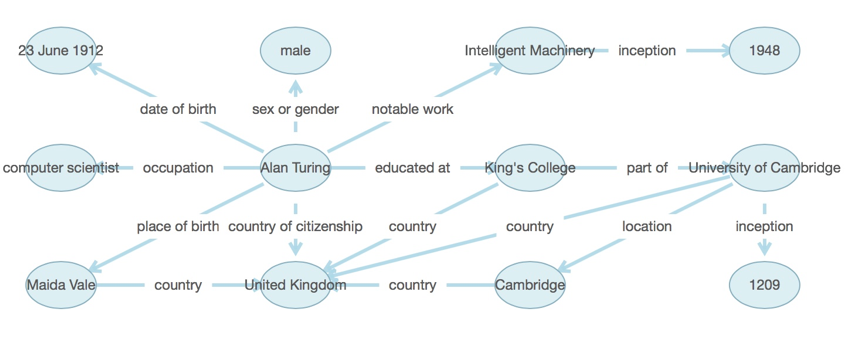
\includegraphics[width=0.80\textwidth]{kg.png}
    \caption{An Example Knowledge Graph}
    \label{fig:kg}
\end{figure}

In our framework, we use knowledge graph as our external knowledge base. As illustrated in Figure\ref{fig:kg}, a knowledge graph contains nodes and relations. The nodes are entities, the arcs are labelled with the relations between those entities. The arrow on the arc indicates the direction of the relation. There are many advantages for using knowledge graphs as the external knowledge:


\begin{figure}[h]
    \centering
    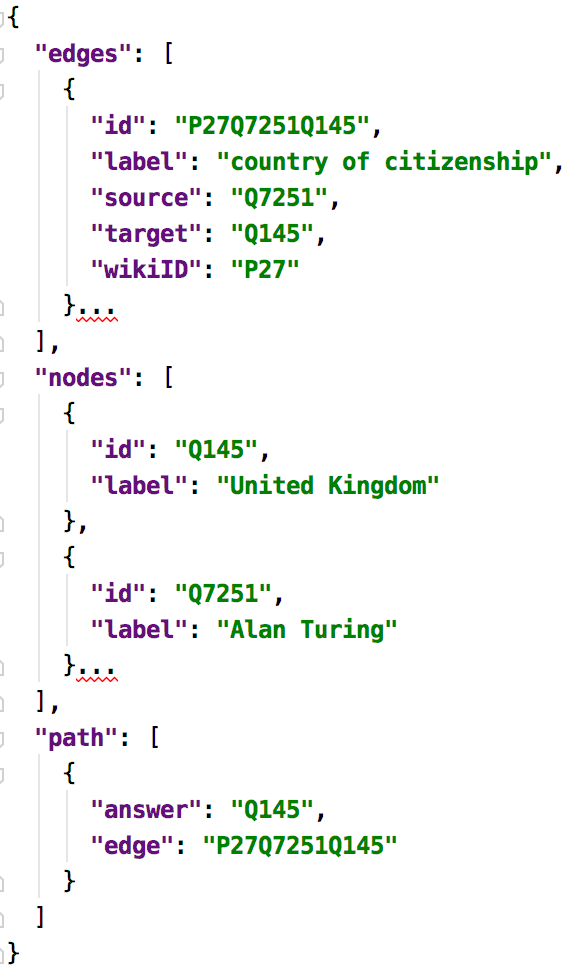
\includegraphics[width=0.4\textwidth]{gkjson.png}
    \caption{An Example Knowledge Graph in JSON Format}
    \label{fig:kgjson}
\end{figure}

\begin{enumerate}
   \item Knowledge graph have two modalities.
   
   As demonstrated in Figure\ref{fig:kgjson}, knowledge graph can be stored as structural data in the computer memory or visualized as an image graph. These two representations convey exactly the same information with different modalities. This provides both machine-readability and human-readability.
   
   \item Knowledge graphs are unambiguous.
   
   Different people have different way to interpret a sentence and label a text span. This makes the evaluation of the Question-answering task very challenging. As I mentioned above, human usually under-perform under such tasks. Unlike plain text, knowledge graph is unambiguous wich make the evaluation more accurate.
   
   \item  Knowledge graphs are structural.
   
   Knowledge graph are structural in the sense that the relations between entities are easily interpretable. This makes it extremely easy to control the topic and topic switch of the conversations.

    
    \item Knowledge graphs are open domain.
    
    There are many existing knowledge graph datasets\cite{vrandevcic2014wikidata,bollacker2008freebase}. These knowledge graphs covers a wide range of topics which could be considered open-domain.
    
    \item Knowledge graphs are well-studied.
    
    There are many prior works related to knowledge graphs, such as embedding\cite{lin2015learning}, which could be useful for developing our own system. In addition, a knowledge graph is a directed graph, there are many algorithms, such as depth-first search, we could use for many purposes, such as sampling a sub-graph from the whole graph.

\end{enumerate}

As outlined above, knowledge graphs seem to be a good resource of external knowledge in our task. There are two popularly knowledge graphs which are widely used in literature, we decide to use WikiData\cite{vrandevcic2014wikidata} instead of Freebase\cite{bollacker2008freebase}. WikiData has a running API which researchers could query the API directly instead of dealing with raw data.

\subsection{Natural Conversation Grounded on Knowledge Graph}

In our framework, we sample sub-graphs from Wikidata. Each graph contains 12 nodes and all these nodes are connected via edges. Each edge annotates the relations between these nodes. For each conversation, there will be 6 relations and answer nodes highlighted in sequence. For each turn, there will be a new relations and answer node highlighted, however, the rest graph remain the same. The sequence of highlighting relations (path) is predefined in order to control the topic switches in the conversation. Here\ref{tab:terms}, I would like to introduce some terminologies before we demonstrating different types of sampled graphs.

\begin{table}[]
\begin{tabular}{|l|l|}
\hline
Terms         & Definition                                                                                                                                                                                                                       \\ \hline
Gaps          & \begin{tabular}[c]{@{}l@{}}If there is no overlap between the entities in relations between the previous \\ turn and the current turn, then we label the current turn with ‘Gap’ label.\end{tabular}                             \\ \hline
Continuous    & A conversation with no gap is called continuous.                                                                                                                                                                                 \\ \hline
Discontinuous & A conversation with one or more gaps is called continuous.                                                                                                                                                                       \\ \hline
Links         & \begin{tabular}[c]{@{}l@{}}When two turns are talking about the same entity, we call the following \\ turn is linked to the previous turn if there is a strong correlation between \\ their grounded relationships.\end{tabular} \\ \hline
\end{tabular}
\caption{Definition for Graph Annotation}
\label{tab:terms}
\end{table}

We sampled 10 sub graphs from Wikidata in 10 distinct topics. For each subgraph, we generate 4 paths for each graph with different number of gaps and links in the path. By doing this, we would like to investigate under what situation, human tend to produce various linguistic patterns, particularly elided construction, in an extended coherent dialogue.


\begin{figure}[h]
    \centering
    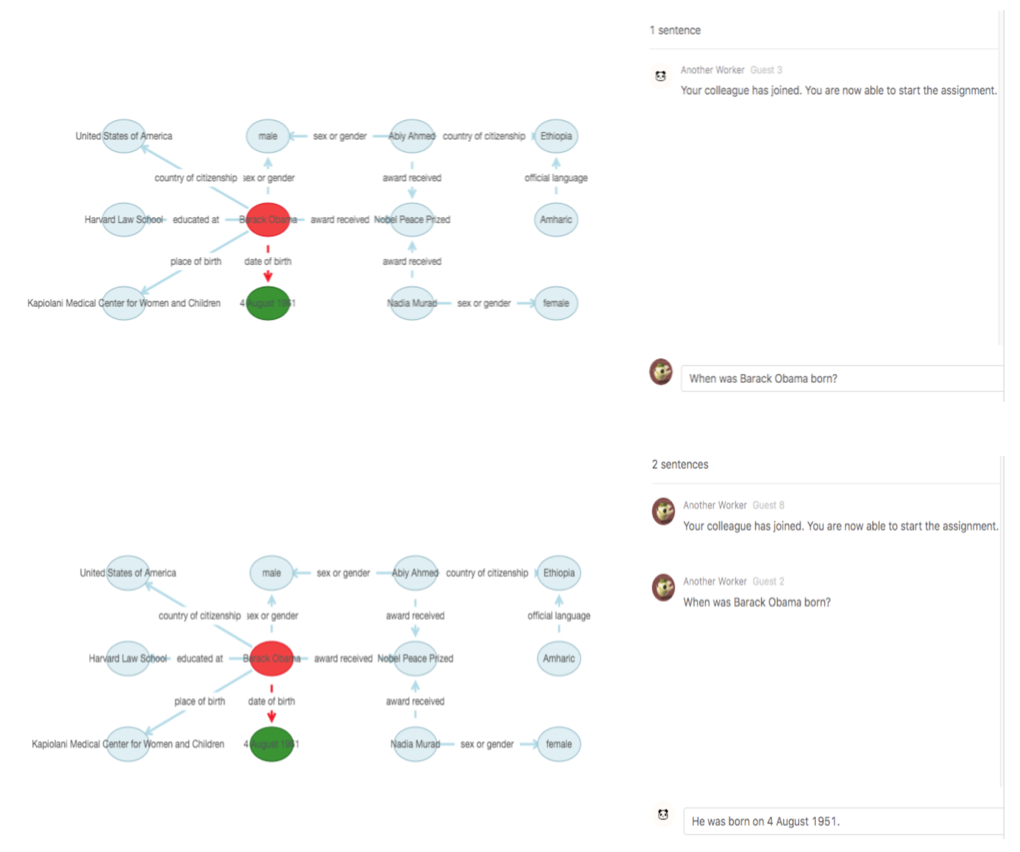
\includegraphics[width=0.8\textwidth]{qa1.png}
    \caption{Questioner(above) and Answerer(below) Interface for Question Answering Task.}
    \label{fig:kgjson}
\end{figure}


\begin{figure}[h]
    \centering
    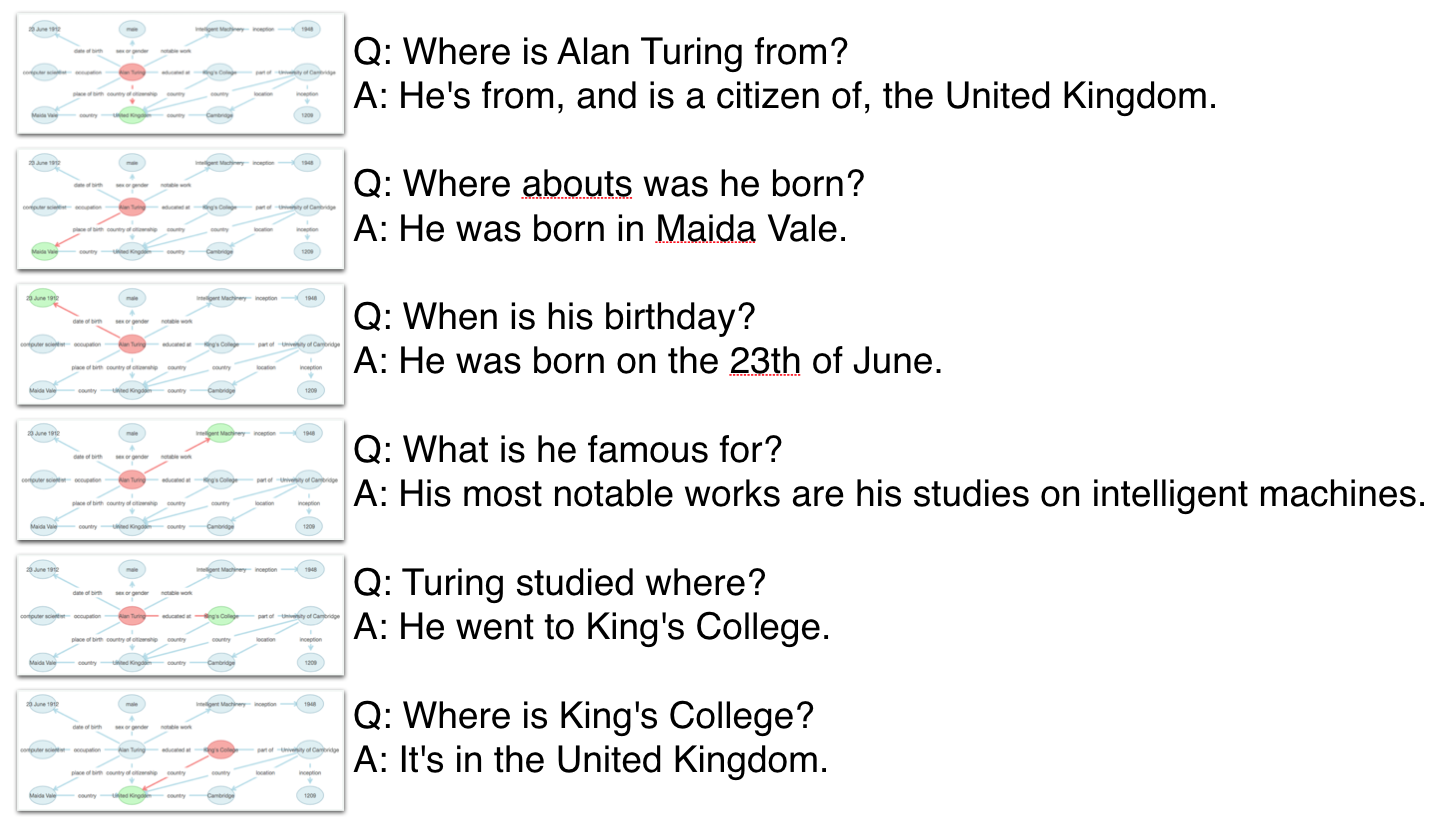
\includegraphics[width=0.8\textwidth]{eaxmppledata.png}
    \caption{An Example Collected Data-point}
    \label{fig:exampledata}
\end{figure}




For each conversation, there are two participants. One is Questioner and the other is Answerer. They will talk in turns. They have freedom to choose how to phrase their sentences and keep the conversation natural, although, what they are talking about is constrained. Questioner is the initiator of the conversation. In order to start a conversation, Questioner should ask a question based on the relation (arc) in RED. The node marked in GREEN should be the answer of the question. Answerer will receive the question from the Questioner together with the same graph and the same marking and he/she has to give a response which is the answer to that question. After Questioner received the response from Answerer, the graph will be updated automatically. Then Questioner could ask one more question to keep the conversation going naturally and the whole process will be repeated for 6 turns. During the experiment, participants should not see each other, because no-vocable commutation could influence the experiment outcome. There is no other hard constrain in our task, because we would like to keep the conversation as natural as possible.



Each conversation is linked with the subgraph it grounded on. Within the conversation, each question-answering pair is linked with the highlighted relation and node in the knowledge graph. In addition, some demographic information about the participants, such as age, gender and nationalities, os also collection under their permission. Here is an example of collected data-point\ref{fig:exampledata}.





\subsection{Annotations for Linguistics Patterns}

Each utterance is labelled with various linguistics patterns by human annotators. There are five labels in our datast. Four of them are considered to be classification tasks, which the annotator see the whole utterance and decide if the sentence contains such a pattern. The rest four tags are considered to be sequence labelling tasks, which these tags are labeled to a text span of the original utterance. Table\ref{tab:tags} summarize the details about our tag set. In addition, you could find more details about the tag set in the annotation schema in appendix.




% Please add the following required packages to your document preamble:
% \usepackage{multirow}
% \usepackage{graphicx}
\begin{table}[]
\centering
\resizebox{\textwidth}{!}{%
\begin{tabular}{|l|l|l|}
\hline
Type                            & Tag                                                                            & Definition                                                                                                                                                                                                                                                                                                                                                                                                                                                                                                       \\ \hline
\multirow{4}{*}{Classification} & Sluicing                                                                       & \begin{tabular}[c]{@{}l@{}}Sluicing is a type of ellipsis that occurs in both\\ direct and indirect interrogative clauses. The ellipsis\\ is introduced by a wh-expression, whereby in most\\ cases, everything except the wh-expression is elided\\ from the clause.\end{tabular}                                                                                                                                                                                                                               \\ \cline{2-3} 
                                & Anaphor                                                                        & \begin{tabular}[c]{@{}l@{}}Anaphora is the use of an expression whose\\ interpretation depends upon another expression in \\ context (its antecedent or postcedent). In our schema,\\ anaphora is the use of an expression that depends\\ specifically upon an antecedent expression.\end{tabular}                                                                                                                                                                                                               \\ \cline{2-3} 
                                & Short Answer                                                                   & \begin{tabular}[c]{@{}l@{}}Short answer (= answer fragments) is a type of\\ ellipsis that occurs in answers to questions. In\\ our schema, we define all answer utterances which\\ is not a fully grammatical sentence to be short answer.\end{tabular}                                                                                                                                                                                                                                                          \\ \cline{2-3} 
                                & Error                                                                          & \begin{tabular}[c]{@{}l@{}}Error tag should only be annotated when there is a\\ disagreement between the grounded knowledge graph\\ and the utterances.\end{tabular}                                                                                                                                                                                                                                                                                                                                             \\ \hline
\multirow{4}{*}{Labelling}      & \begin{tabular}[c]{@{}l@{}}Additional information\\ outside graph\end{tabular} & \begin{tabular}[c]{@{}l@{}}If parts of an utterance introduce additional information\\ into the conversation which is not mentioned in the\\ grounded knowledge graph, we call this part additional\\ information outside the knowledge graph.\end{tabular}                                                                                                                                                                                                                                                      \\ \cline{2-3} 
                                & \begin{tabular}[c]{@{}l@{}}Additional information\\ within graph\end{tabular}  & \begin{tabular}[c]{@{}l@{}}If parts of an utterance introduce additional information\\ into the conversation which is mentioned in the graph\\ and such information is not highlighted, we call them\\ additional information within the knowledge graph.\end{tabular}                                                                                                                                                                                                                                           \\ \cline{2-3} 
                                & Conversation Control                                                           & \begin{tabular}[c]{@{}l@{}}Conversation Control label should be tagged to any\\ pieces of utterance which functionally act as a\\ connector to make the whole conversation more\\ natural and coherent.\end{tabular}                                                                                                                                                                                                                                                                                             \\ \cline{2-3} 
                                & Totally Irrelevant                                                             & \begin{tabular}[c]{@{}l@{}}Totally irrelevant tag should be used when pieces of\\ utterance is totally irrelevant to the question answering\\ conversation. By deleting such pieces of information,\\ we will not influence the coherence of the conversation\\ or the meaning of the utterance. In addition, this tag should\\ only be considered if the part of utterance is not labelled as\\ other labels. In other words, labels, such as Conversation\\ Control, will have higher precedence.\end{tabular} \\ \hline
\end{tabular}%
}
\caption{Definition of Tag Set.}
\label{tab:tags}
\end{table}



\newpage





\section{Implementation}

In this section, I would introduce the tool-kits I have developed and used during this project. I will also mentioned the publicly available packages I have adapted for the development.

\subsection{Sampling from Knowledge Graph}

In order sample sub-graphs from Wikidata, a Java toolkit named KnowledgeGraphClient is developed.

\begin{figure}[h]
    \centering
    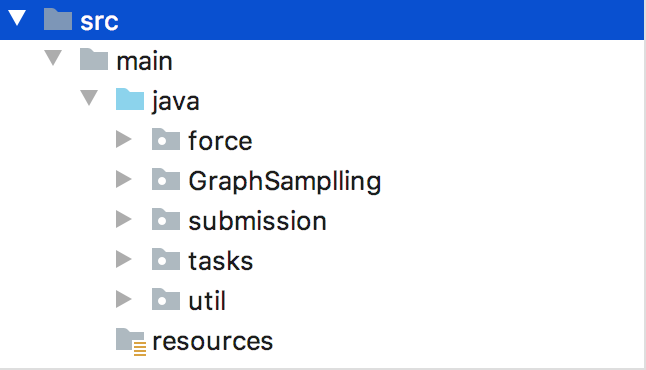
\includegraphics[width=0.4\textwidth]{client.png}
    \caption{Structure of KnowledgeGraphClient.}
    \label{fig:client}
\end{figure}

In order to interact with Wikidata, a Java package name Wikidata Toolkit\cite{wikitoolkit} is used. This package provide APIs to query Wikidata for entities (nodes in Figure\ref{fig:kg}) and relations relation to it.

A sub-graph is sampled from via a depth-first search algorithm. We pre-defined a set of "interesting relations" which we only explore next connected node if the relation is in that set. We clearly don't want to include relations which are rarely mentioned in our daily life. For example, we would rarely talk about relations like: Obama is an instance of human and human is a sub lass of animal. We start the search at a predefined node, for example, Obama(Q76). Q76 is the unique Wikidata ID for Obama. We potentially could traversal all nodes which are connected with Obama, however, I set the maxmim depth of the search to be 2. After the search, we would have a set of edges an nodes which will form a directed graph. In order to visualise the graph, I applied force-directed algorithm to make reduce the overlap among nodes.

\begin{figure}[h]
    \centering
    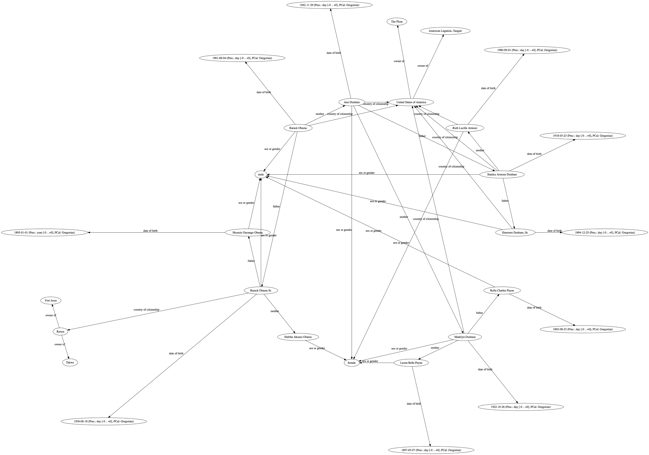
\includegraphics[width=0.4\textwidth]{obama.png}
    \caption{An Example Force-Directed Graph.}
    \label{fig:obama}
\end{figure}

However, such a graph is not very human interpretable. I decided to follow a semi-automatic approach which I manually select nodes and edges from the above graph and directly give x and y indexes of each node. In addition, the paths are also manually generated. By this approach, I generated 40 graphs in 10 distinct topics.

\subsection{Generating Questions from Knowledge Graph}

Instead of collecting dialogues from human partiancipants, Indurthi et al.\cite{indurthi2017generating} has try to automatically generate question answer pairs from a given knowledge graph. 

They first extract a set of keywords from entities and relationships expressed in a triple stored in the knowledge graph. From each such set, we use a subset of keywords to generate a natural language question that has a unique answer. They treat this subset of keywords as a sequence and use an encoder-decoder model to generate natural questions from it. I re-implemented their experiment in a similar setting and my experiment results are shown in table\ref{tab:genresult}. The larger model is a bi-directional RNN containing one hidden layer of 1000 units. I also build a small model, use a bi-directional RNN containing one hidden layer of 500 units due to the limitation of computation power. However, their method faces domain-adaption problem which could not produce grammatical sentences with out-domain data. Consequently, this dataset requires human intelligence which crowdsourcing is needed. 

\begin{table}[]
\centering
\begin{tabular}{|l|l|}
\hline
Models                 & BLEU Score \\ \hline
BiRNN-Large-Reported   & 50.14      \\ \hline
BiRNN-Small-Experiment & 38.45      \\ \hline
BiRNN-Large-Experiment & 49.72      \\ \hline
\end{tabular}
\caption{Experiment Result for Generating Conversation\cite{indurthi2017generating}}
\label{tab:genresult}
\end{table}

\subsection{Web-interface for Data Collection}

In order to collect this corpus via crowd-sourcing, I built a web-interface together with a web server from scratch. A large proportion of my effort have been spent into developing these software. There are two major challenges: 1) This is a production system, which real users have to interact with this system. Consequently, the system has to be thoroughly tested. 2) Sometimes, human behaviour are unpredictable. Because this system is directly interact with humans, it's very challenging to design the system in order to achieve desired results.

\begin{figure}[h]
    \centering
    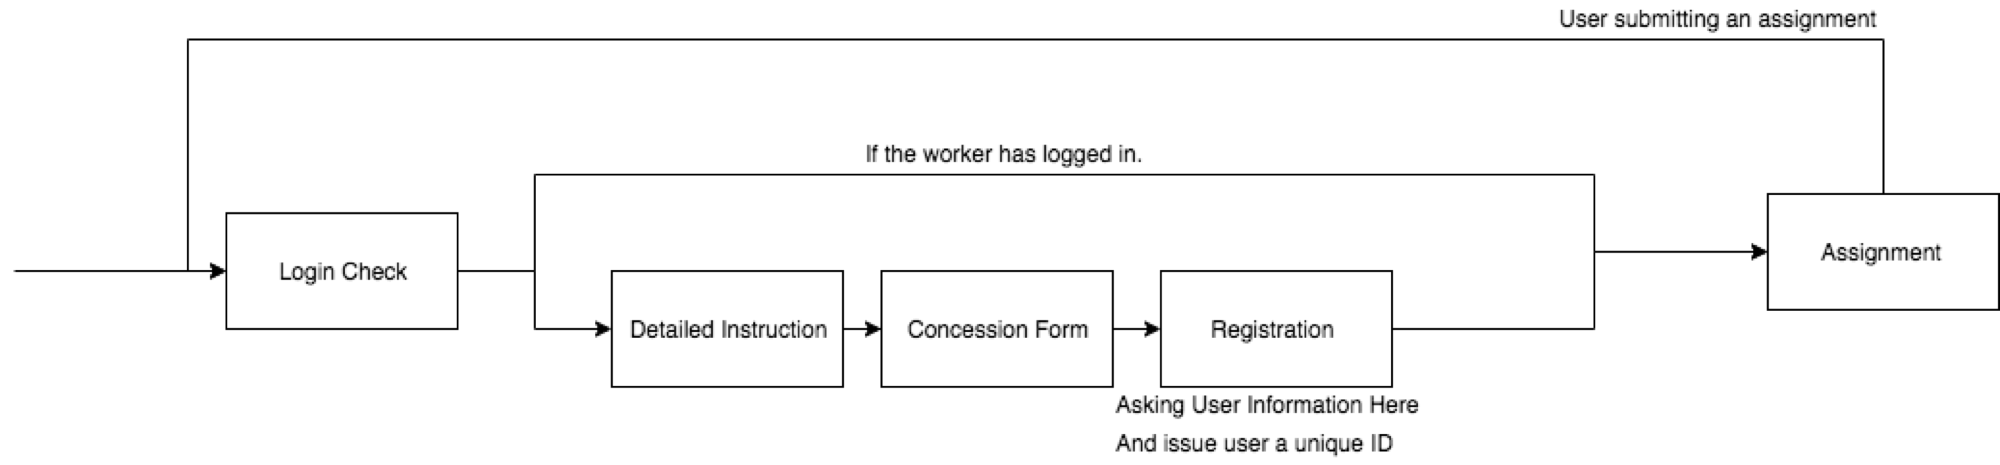
\includegraphics[width=0.9\textwidth]{process.png}
    \caption{The Workflow of the Web Interface.}
    \label{fig:web}
\end{figure}

As shown in Figure\ref{fig:web}, if a new user participates in our experiment, he/she will be shown a detailed instruction about the experiment. If the participant decides to take part in the experiment, he/she has to sign a consent form according to the data protection regulation. If the user agree with terms and conditions of the experiment, after registering an account, the user could see the web-page for the task. More detailed workflow and screen shots are in appendix. In order to develop this web interface, I have used many packages.

\begin{table}[]
\centering
\begin{tabular}{|l|l|}
\hline
Package                  & Purpose                                                   \\ \hline
NodeJS\cite{nodejs}      & Writing Web-server.                                       \\ \hline
MongoDB\cite{monodb}     & Database for storing user information and collected data. \\ \hline
ReactJS\cite{react}      & Build user interfaces.                                    \\ \hline
AntD\cite{antd}           & Important components for user interface.                  \\ \hline
G6\cite{g6}              & Rendering knowledge graphs in frontend.                   \\ \hline
Socket.IO\cite{socketio} & Writing socket server for online chatting.                \\ \hline
\end{tabular}
\caption{Packages Imported for Developing the Web-interface.}
\label{tab:packages}
\end{table}



\subsubsection{Tools for Annotating the Dataset}

In order to annotate the dataset, a toolkit named doccano\cite{doccano} is used. This is a easy to use web application which provides features for sequence to sequences task, classification task and sequence labelling task. I have played with many annotation tools, most of them are professional and complicated to set up.

In addition, I develop a tool for post-processing and parsing our corpus which is frequently used during my data analysis.

\begin{figure}[h]
    \centering
    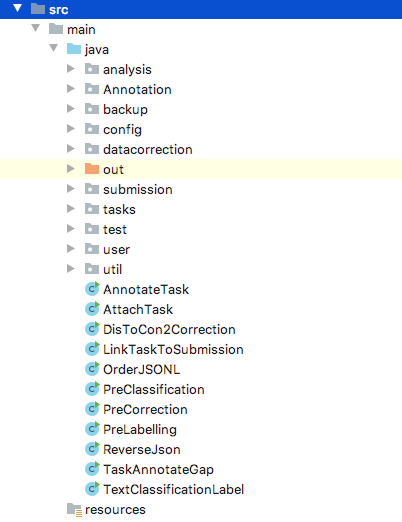
\includegraphics[width=0.4\textwidth]{parser.png}
    \caption{Toolkit for Post-processing and Parsing the Dataset.}
    \label{fig:parser}
\end{figure}



\newpage
\section{Data Collection Procedure}

In this section, I introduce how the corpus is collected. The whole data collection experiment runs for 2 months which is the most challenging and time-consuming part for this project. These are several constrains of this experiment which makes organizing and organizing this experiment extremely hard. During the experiment, I have organized totally 30 sessions. The project is funded by Informatics Student Service and each participant will be paid a 5 pounds Amazon Voucher.

\begin{enumerate}
   \item Each experiment session need two participants at the same time. 

   \item Only native speakers could participate in this experiment.
 
   \item Building a robust system that multiple users could interact simultaneously is hard. 
       
\end{enumerate}

In this section, I discuss our data collection procedure in the following order: Advertising the Experiment, Scheduling the Experiment and Paying the participants. Finally, I would like to give some advises for futures researchers who are aiming to collect a dialogue corpus in lager scale. 


\subsubsection*{Advertising the Experiment}

In order to recruit enough participants in this project, advertising this experiment is crucial. I have try several methods.

\begin{enumerate}
   \item Email the whole Informatics students.

   \item Pin leaflet around the camps. 
 
   \item Posting advertisement on social medial (Facebook).
\end{enumerate}

Emailing students is the most effective approach which I recruit most of the participant from. An alternative is approach is to deploy the task to crowdsourcing platform, such as Amazon Mechanic Turk\cite{mturk}.  Based on my own experience, we are able to recruit hundreds of participants overnight.


\subsubsection*{Scheduling the Experiment}

The most challenging part of the data collection and even the whole project is to schedule the sessions. It is very difficult pair up the participants and find a suitable time for both of them. I have tried to make a google form and ask participants to select in their available time. Or I have send all the interested participants a group email and ask them if they have time for a fix-time session. Because not all people check their email regularly, it takes time for our participants to reply. Consequently, all of the above approaches don't work well enough.

Finally, I start follow the following procedural which works reasonably well. 

\begin{enumerate}
   \item Build an online survey to ask roughly when are they available next week.

   \item Pair up participants who are available on the same data.
 
   \item Ask permission to share their email with other participants.
   
    \item Ask permission to share their email with other participants.

    \item Send them a group email and ask them to find a suitable time for the experiment session.

    \item Confirm the attendance one day before the experiment and send them detailed instruction for the experiment sessions.
    
\end{enumerate}

However, when the scale of the corpus goes larger. I strongly encourage researchers to hire full time in-house annotators, if the resource is available.

\subsubsection*{Payment Method}

All payment are sent via Amazon Vouchers.


\section{Data Annotation Procedure}

The whole corpus is annotated by in-house annotators (my friends and I) according to an Annotation Schema (See Appendix). The majority of the annotation work is done by myself. A subset of the corpus (10\%) has been annotated twice by different annotators, in order to calculate the inter-annotator agreement. Cohen's Kappa is used for calculate agreement between annotators.

\section{Compare to Previous Work}

Our corpus contains natural extended conversations grounded on an external wide-coverage structural knowledge graph. At present, there are no such datasets exist (see Table\ref{tab:compare}) and this is what our dataset is mainly developed for.

% Please add the following required packages to your document preamble:
% \usepackage{graphicx}
\begin{table}[]
\centering
\resizebox{\textwidth}{!}{%
\begin{tabular}{|l|l|l|l|l|l|}
\hline
Dataset                           & Year & Multi-turn & Natural Conversation & Answer Type           & External Knowledge Type \\ \hline
CoQA\cite{reddy2019coqa}          & 2018 & \bluecheck & \bluecheck           & Text Span             & Text                    \\
CSQA\cite{saha2018complex}        & 2018 & \bluecheck & \xmark               & Text Answer           & Knowledge Graph         \\
SQuAD\cite{rajpurkar2016squad}    & 2016 & \xmark     & \xmark               & Text Span             & Wikipedia articles      \\
SQuAD 2.0\cite{rajpurkar2018know} & 2016 & \xmark     & \xmark               & Text Span             & Wikipedia articles      \\
QuAC\cite{choi2018quac}           & 2018 & \bluecheck & \xmark               & Text Span             & Wikipedia articles      \\
FiloIT\cite{shekhar2017foil}      & 2017 & \xmark     & \xmark               & Text Span             & Images                  \\
GuessWhat\cite{de2017guesswhat}   & 2017 & \bluecheck & \xmark               & Object Position       & Images                  \\ \hline
Our Dataset                       & 2020 & \bluecheck & \bluecheck           & Natural Text Response & Knowledge Graph         \\ \hline
\end{tabular}%
}
\caption{A Comparison between this Dataset with Existing Related Question Answering Datasets.}
\label{tab:compare}
\end{table}






\chapter{Analysis and Discussion}

In this chapter, we perform some quantitative and qualitative analysis based on our corpus. We made several hypothesis according to our observation and we statistically test their significance using t-test.

\section{Summary of the Corpus}

In previous chapter, we introduce a novel conversational question answering dataset. Our dataset contains 240 natural conversations, each has 6 question-answering pairs, in 10 distinct topics. These Conversations are divided into two categories: continuous and discontinuous. There are 140 continuous and 100 discontinues conversations. Discontinues conversations are additionally split into two subgroup, dis1 (conversation with only one gap) and "Dis2" (conversations with many gaps). There are 43 "dis1" conversations and 57 "dis2" conversations. A detailed count for each topics is shown in Table\ref{tab:topiccount}. Table\ref{tab:datacount} shows various count about the data set. 

% Please add the following required packages to your document preamble:
% \usepackage{graphicx}
\begin{table}[]
\resizebox{\textwidth}{!}{%
\begin{tabular}{|l|l|l|l|l|}
\hline
Topics             & WikiData ID & Continuous & Discontinuous1 & Discontinuous2 \\ \hline
AlanTuring         & Q7251       & 13         & 6              & 5              \\ \hline
JKRowlin           & Q34660      & 14         & 6              & 6              \\ \hline
Knuth              & Q17457      & 19         & 0              & 6              \\ \hline
Obama              & Q76         & 9          & 5              & 6              \\ \hline
Berkshire Hathaway & Q217583     & 12         & 7              & 5              \\ \hline
Softbank           & Q201653     & 18         & 0              & 6              \\ \hline
Apple              & Q312        & 11         & 7              & 6              \\ \hline
CPU                & Q5300       & 19         & 0              & 7              \\ \hline
London             & Q84         & 12         & 5              & 6              \\ \hline
Tianjin            & Q1173       & 13         & 6              & 5              \\ \hline
\end{tabular}%
}
\caption{Detailed Topics Count for the Corpus.}
\label{tab:topiccount}
\end{table}


\begin{table}[]
\centering
\begin{tabular}{|l|l|}
\hline
Number of Dialogues & 240   \\ \hline
Number of Questions & 2.9K  \\ \hline
Number of Answers   & 2.9K  \\ \hline
Number of Words     & 1.8K  \\ \hline
Number of Tokens    & 15.2K \\ \hline
\end{tabular}
\caption{Counts of the Dataset.}
\label{tab:datacount}
\end{table}


\subsection{Inter-Annotator Agreement of the Corpus}

Inter-annotator agreement is a measure of how well two (or more) annotators can make the same annotation decision for a certain category. Cohen's Kappa is used here for calculating the agreement score between two annotators.

\begin{table}[]
\centering
\begin{tabular}{|l|l|l|}
\hline
Tag                                                                            & Cohen's Kappa & Aggrement                \\ \hline
Anaphora                                                                       & 0.9476        & Almost perfect agreement \\ \hline
\begin{tabular}[c]{@{}l@{}}Short\\ Answer\end{tabular}                         & 0.9370        & Almost perfect agreement \\ \hline
Error                                                                          & 0.0           & Slight agreement         \\ \hline
Sluicing                                                                       & 0.0           & Slight agreement         \\ \hline
\begin{tabular}[c]{@{}l@{}}Totally\\ Irrelevant\end{tabular}                   & 0.0           & Slight agreement         \\ \hline
\begin{tabular}[c]{@{}l@{}}Additional\\ information outside graph\end{tabular} & 0.3405        & Fair agreement           \\ \hline
\begin{tabular}[c]{@{}l@{}}Additional\\ information within graph\end{tabular}  & invalid       & Poor agreement           \\ \hline
\begin{tabular}[c]{@{}l@{}}Conversation\\ Control\end{tabular}                 & 0.6060        & Moderate agreement       \\ \hline
\end{tabular}
\caption{Inter-annotator Agreement of the Corpus}
\label{tab:agree}
\end{table}

According to Table\ref{tab:agree}, Anaphora and Short Answer have a almost perfect agreement. The main reason is that the definition of these two tags are relative disambiguate,    










\chapter{Modelling Coherent Dialogues Using Neural Networks}


In order to encode a coherent dialogue, we need to model long-distance dependencies not only between words in one utterance, but also between sentences within the discourse. For example, in order to model an elided construction, our model has to infer the omission from the longer prior context of the conversation, because such information may not appear in the current utterance. To model that, I propose a hierarchical attentional encoder which is inspired by Xing et al. \cite{xing2018hierarchical}. I extend their model with context windows which the size of the windows is a predefined hyper-parameter to control how many previous turns we are modelling. 


\begin{figure}[h]
    \centering
    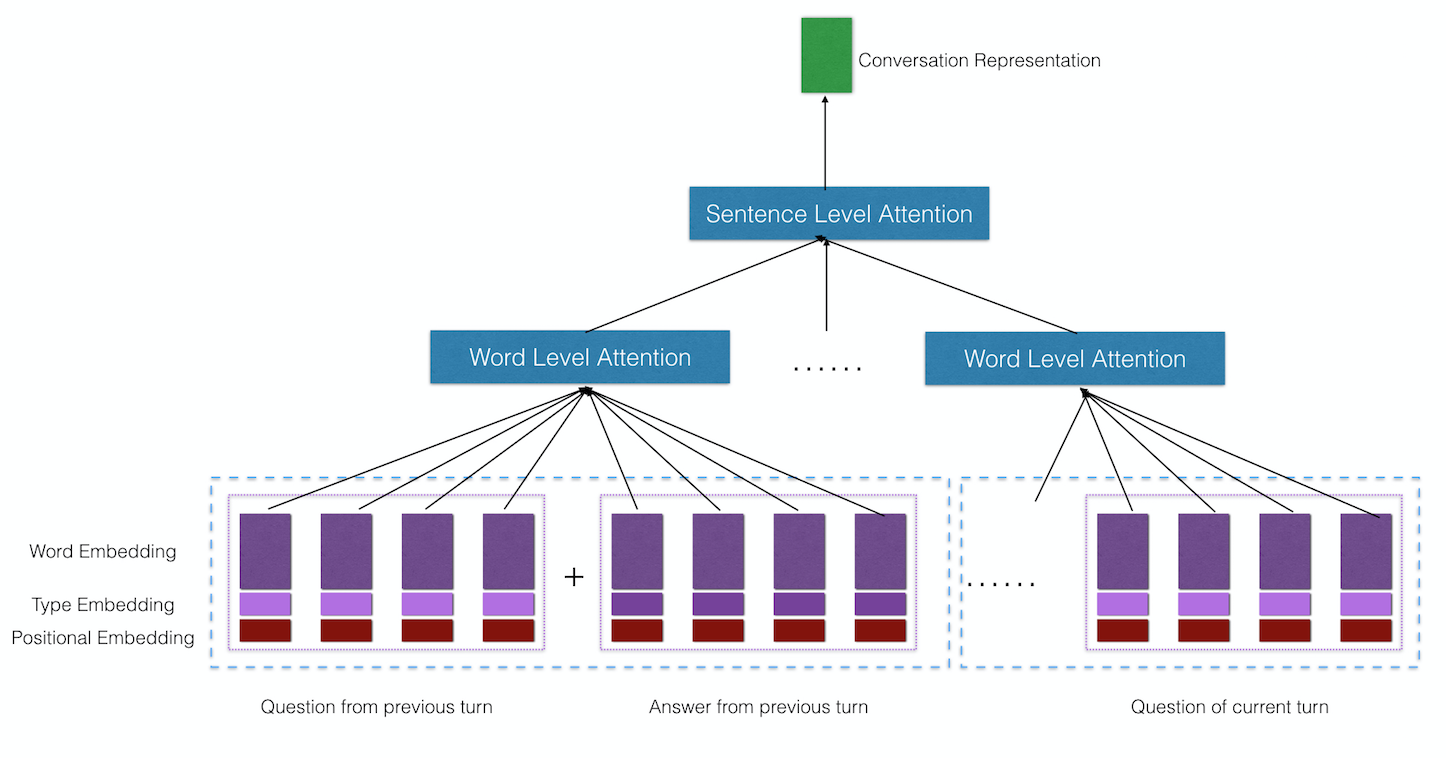
\includegraphics[width=0.75\textwidth]{attemodel.png}
    \caption{Hierarchical Attentional Encoder with Context Window.}
    \label{fig:mesh1}
\end{figure}

I would like to use BERT\cite{devlin2018bert} to provide a contextual embedding for each word. Additional turn embedding is used to denote the turn and type of a sentence. The concatenated embedding is fed into a self-attentional layer which models the dependencies within the context window. Additional sentence level attention will be used to model the dependencies between context windows. In addition, I will adapt a multi-modal deep neural network architecture to produce the dialogue state representation for downstream tasks.

\begin{figure}[h]
    \centering
    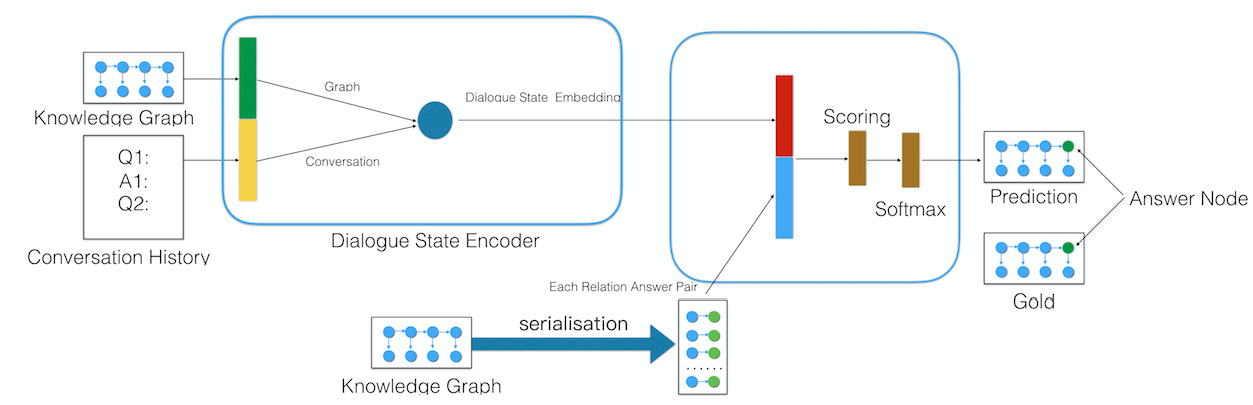
\includegraphics[width=0.85\textwidth]{qa1pro.png}
    \caption{The Multi-modal Question Answering Architecture.}
    \label{fig:mesh1}
\end{figure}

To predict the correct node to answer a given question, we could represent a prediction as a quadruple, such as, (Subject Node, Relation, Object Node, Position of the Answer). An example of the prediction could be (Barack Obama, born, 1967, object) which corresponds to the question ``When was Obama born?". I permute all the possible combinations within the graph. Then I use a feed-forward neural network together with a softmax layer to produce a multinomial distribution over all the possible answers. Then the prediction is compared with the gold answer and we could calculate the reward or loss to train our model.

\subsection{Generate coherent dialogues as a Markov decision process}
\noindent
As I argued above, training a dialogue system with supervised learning is not explicitly optimized to produce a coherent response. I propose to cast the response generation task as a RL task. More specifically, I consider the questioner and the answerer as part of the RL agent environment. According to Williams and Young\cite{williams2007partially}, a goal-driven dialogue system could be modelled as a partially observable Markov decision process. Inspired by Strub et al. \cite{strub2017end}, I would like to describe our response generation task as following:

I define the state $S_t$ as the state of the dialogue at step t. An action $u_t$ corresponds to selecting a new word in the vocabulary V. The transition to the next state depends on the selected action:

\begin{itemize}
\item If we generate the end of sentence token . , the ongoing response is terminated and the next question is sampled from the questioner.
\item Otherwise the new word is appended to the ongoing answer.
\end{itemize}

A dialogue is started with an initial question and finished after a fixed number of turns. A reward is defined for every state action pair. 

\subsection{Extrinsic evaluation of dialogue models}
\noindent
I will use precision and recall, which are well-established metrics for question answering tasks, as our extrinsic evaluation metrics. In my framework, high precision and recall demonstrate a good performance of modelling the linguistic patterns within a coherent dialogue.





\chapter{Conclusion and Future Work}




Current statistical spoken dialogue systems (hereafter SDSs) have three key components which are shown as Figure \ref{fig:sds}. Semantics decoder decodes the meaning in utterances into dialogue acts which describe the current intention of the user, for example, confirm(food=Korean). Then, dialogue manager, which usually consists of a belief tracker and a policy network, will keep track of the belief states and produce a dialogue act as the response. Later a semantic encoder (natural language generator) will map this act back into natural language. Although the current statistical SDSs do explicitly capture the dialogue history via belief tracking, they may not utilize rich linguistic information inside a coherent dialogue. I would like to integrate our conversation model into the semantic decoder and encoder to enable the current SDSs to understand and produce more coherent dialogues. In addition, current SDSs require pre-defined ontology in order to keep track of the belief state. I would like to investigate whether we could connect a SDS to a wide coverage knowledge graph and build a dialogue system which can support a natural conversation about any topic within the knowledge graph.

\begin{figure}[h]
    \centering
    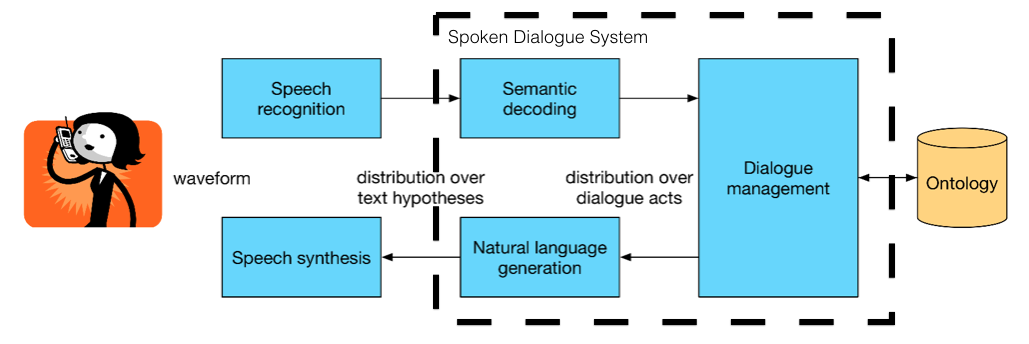
\includegraphics[width=0.80\textwidth]{sds.png}
    \caption{Architecture of a Spoken Dialogue System.\cite{gasic}}
    \label{fig:sds}
\end{figure}

Cheng et al.\cite{cheng2019learning} has developed a transition-base neural semantic parser with a generic tree-generation algorithm. By integrating a conversation model with an existing neural semantic parser, we may enable it to perform semantic parsing over an extended coherent dialogue.

% use the following and \cite{} as above if you use BibTeX
% otherwise generate bibtem entries
\bibliographystyle{plain}
\bibliography{mybibfile}

\end{document}